\section{Small Training Data sets(tentative)}
\label{sec: small_data_sets}

\subsection{WHY Small Training Data Sets}
Like prior works\cite{nam2013transfer, ma2012transfer, rahman2012recalling, ryu2014value, zhang2014towards}, the basic HDP method we proposed uses all the instances in feasible data sets as training data to perform KS-test and build defect prediction learners. The straightforward drawback of using all data is that it will take much long time to finish the whole defect prediction process. The observation from our experiments also verifies this: it takes several days on a 24-cores machine to find all possible matched features in KS-test. On the other hand, whether using all the instances from the data set will be helpful and necessary to build defect learners in such transfer learning scenario is still unclear. In CPDP with transfer learning methods, where data size has a big effect on running time, small training data seems more promising if we can get similar or even better prediction performance. Menzies et.al. \cite{menzies2008implications} pointed out that ``performance ceiling'' exists when using static code features to explore defects in software data repositories.  Furthermore, Thurhan et atl.\cite{turhan2009relative} and Fayola et al.\cite{peters2013better} improved the  performance of the CPDP with the same metric set by applying data filtering techniques to select the filtered training data. Therefore, it would be more interesting to investigate whether using small sampled data sets is feasible in heterogeneous defect prediction. Then we did the following experiment.

\begin{figure}[!htp]
	\centering
% 	\vspace{0.5mm}
	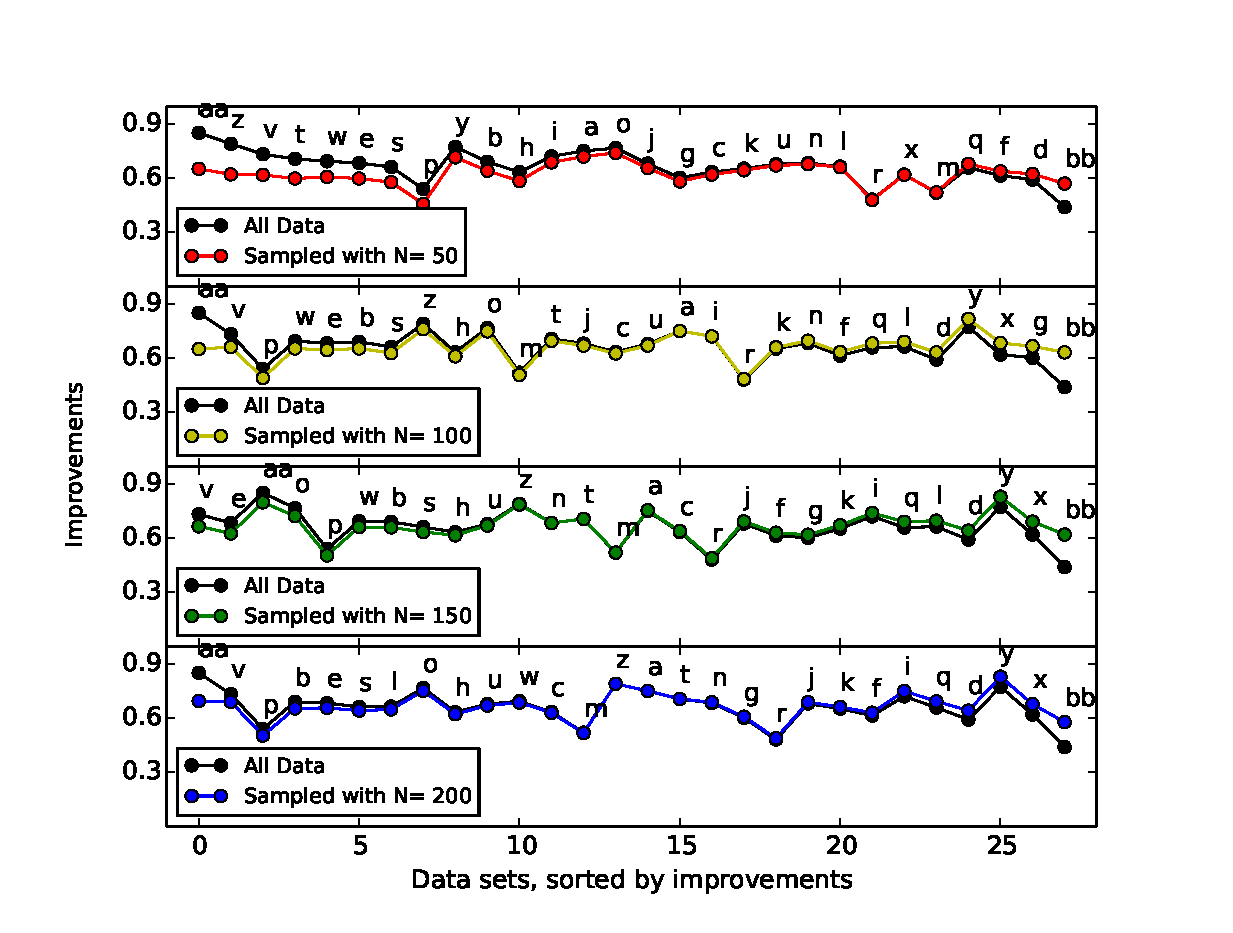
\includegraphics[width=\linewidth]{Figures/raleigh/sample_random.eps}
	\caption{Improvements of using sampled data over all data with sampled size N = \{50, 100, 150, 200\}. We label the data in table \ref{tab:datasets} from a to z, and the last two data sets ar5 and ar6 as aa and bb.}
	\label{fig:small_data}
\end{figure}

\subsection{Approach I}

As mentioned before, data sets are used in two steps in standard HDP besides testing: matching feature and building learner. To evaluate the effect of sample size, instead of using all the instances from candidate data sets, we propose to randomly sample the original data and use smaller data sets for matching features and building learner. For space limitation, we only use KSAnalyzer for matching features.

In this experiment, all the original data sets will be randomly sampled to generate smaller data sets of size $N$, where $N \in \{50, 100, 150, 200\}$. If the number of instances in the original data set is smaller than $N$, all those instances will be included and no sample action is required. Specifically, in KS-test, instead of using original data sets, the sampled smaller data sets will be used. For example, in the original data sets, Apache and arc are with instance size of $194$ and $234$. If KS-test is performed on them, the smaller data sets Apache\_sampled and arc\_sampled will be used, both of which include $N$, say 50, instances. 

After obtaining all the matched features from KS-test, defect prediction learner for the target data set will be built based on the corresponding source data. The similar way is adopted here as in KS-test. Instead of using original data set in the basic HDP method, the previously sampled smaller data set will be used, which is the same sampled source data set used in KS-test. To predict all the defects in the target data sets, the original data set will be used as target. For example, if Apache and arc are source and target data pair according to KS-test result, the smaller Apache\_sampled data with $N$ instances will be used to train the learner, and the original arc with $194$ instances will be the target data to be predicted.

This experiment is conducted over the same data sets as basic HDP with 20 iterations. Logistic regression is the default learner as before. The median of 20 AUCs is reported to evaluate the performance. 
% Since {\it Apahce commons math} library takes quite long time to conduct KS-test as mentioned, we replace it with Scipy, a python package, to speed up our experiment. \footnote{As shown in the table, the difference between those two KS-test results is acceptable}. 
Figure \ref{fig:samll_data} shows the sampled data AUC improvements over original data with $N \in \{50,100,150,200\}$. Note that with the increase of $N$, the difference between all data and sampled data experiment becomes smaller. When $N=200$, $27/28$ tests are within 0.05 difference in terms of AUC and $17/28$ tests show smaller data sets have equivalent or even better performence.



\begin{figure}[!htp]
	\centering
% 	\vspace{0.5mm}
	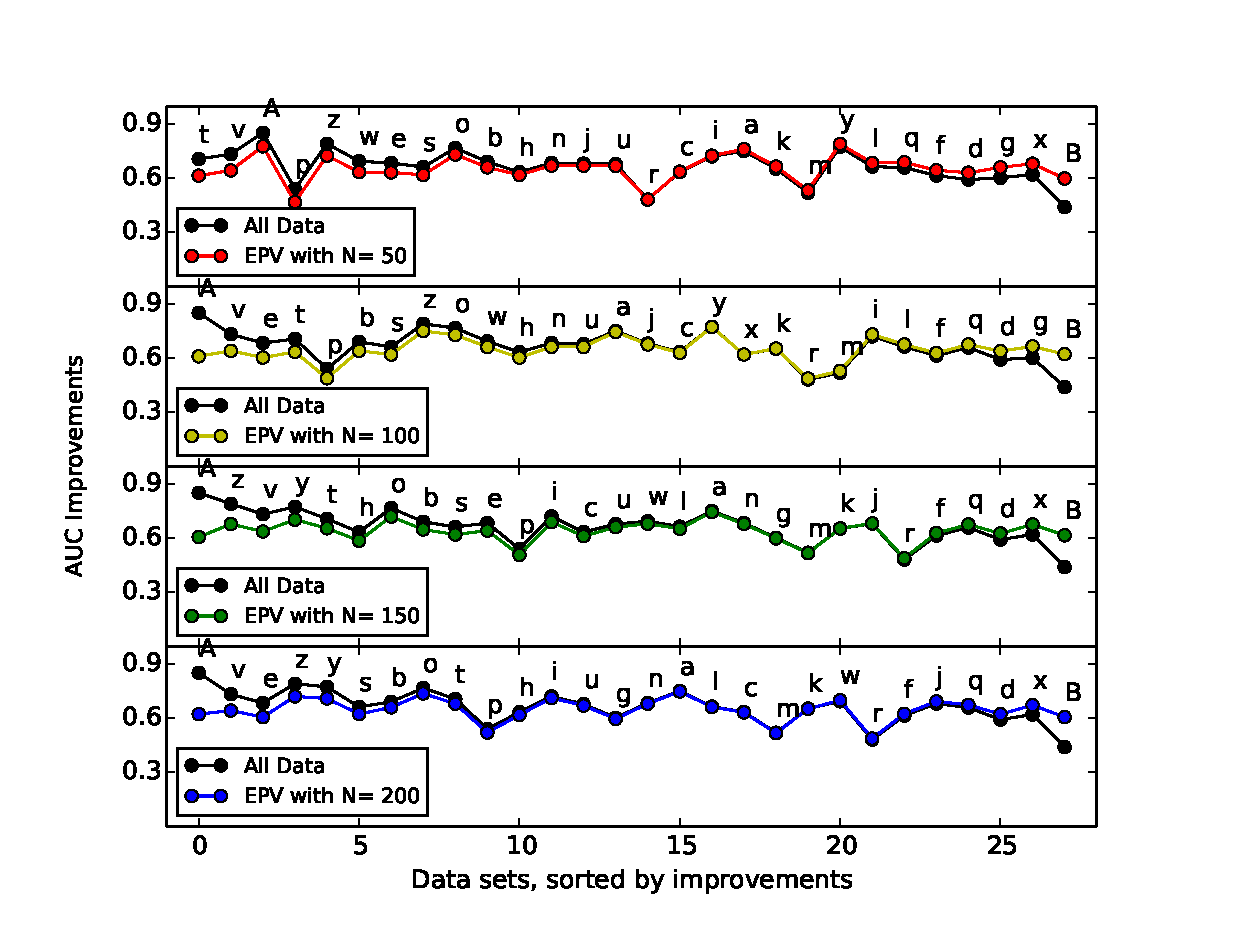
\includegraphics[width=\linewidth]{Figures/raleigh/sample_epv.eps}
	\caption{Improvements of using sampled data N = \{50, 100, 150, 200\} with EPV constraints. We label the data in table \ref{tab:datasets} from a to z, and the last two data sets ar5 and ar6 as aa and bb.}
	\label{fig:small_data}
\end{figure}

\subsection{Approach II}

In \cite{menzies2008implications}, Menzies et al. used Naive Bayes and C4.5 two simple learners to predict defects over PROMISE data. To look for the lower bound on the number of training instances, three sub-sampling techniques were applied to the training data. They found that as few as 50 instances did just as well as larger sample size and 25 might suffice for some data sets. However, in \cite{peduzzi1996simulation}, it was reported that number of events per variable(EPV) would affect the performance of logistic regression. Specifically, if the training data has fewer events relative to the independent variable, the bias of the regression coefficients will be increased.  In HDP method, data sets are used in metric selection, metric matching and learner building, where are exactly we expect to use small data size. The new experiment is designed as fowllowing.

Recall Figure \ref{fig:framework}, for the source data A, instead using all data in Project A, we perform supervised sampling with EPV =10 (recommended in \cite{peduzzi1996simulation})  and N =\{50, 100, 150, 200\} instances will be selected as the new source data ${\hat A}$, which will be used in metric selection, metric matching and prediction phases. For the target project B, instead of using all data for metric matching, a unsupervised sampling applied into project B and resultant data sets ${\hat B}$ with N = \{50, 100, 150, 200\} instances will be only used for metric matching. After prediction model is built with new source data $\hat A$, the original target data B will be applied to predict defects. Note that based on previous HDP experiments, the number of matched metrics(variables) is round 2. Therefore, at most 20 defective instances are randomly selected from source data in supervised sampling.

\subsection{Discussion}
As seen in Figure \ref{fig:small_data}, we can get the similar performance as the original experiment even with the only subset of the original data sets. As $N$ increases from 50 to 200, the performance doesn't change a lot.


